\subsection{Data Processing and Methods}\label{subsection_data_processing_and_methods}

\subsection{Charts}

\begin{table}
    \centering
    \caption{Dataset of Origin of Selected Regressors}\label{regressor_origin}
    \begin{tabular}{| l || c |}
    \hline
    regressor\_name &          dataset \\
    \hline
    \hline
    median\_rooms &  characteristics \\ \hline
    educ\_nohs &  characteristics \\ \hline
    white &  characteristics \\ \hline
    mean\_cash\_public\_assistance\_income\_dollars &  characteristics \\ \hline
    per\_capita\_income\_dollars &  characteristics \\ \hline
    median\_household\_income\_dollars &  characteristics \\ \hline
    part of educ\_further &  characteristics \\ \hline
    mean\_retirement\_income\_dollars &  characteristics \\ \hline
    median\_age\_years &  characteristics \\ \hline
    mean\_travel\_time\_to\_work\_minutes &  characteristics \\ \hline
    homeowner\_vacancy\_rate &  characteristics \\ \hline
    move\_post2010 &  characteristics \\ \hline
    average\_household\_size &  characteristics \\ \hline
    english\_prof\_pct &             educ \\ \hline
    math\_prof\_pct &             educ \\ \hline
    construction &              gdp \\ \hline
    edian\_listing\_price &           h\_vals \\ \hline
    median\_square\_feet &           h\_vals \\ \hline
    median\_days\_on\_market &           h\_vals \\ \hline
    nlocal\_ibs &        n\_ibuyers \\ \hline
    ntop\_ibs &        n\_ibuyers \\ \hline
    rnaturalinc &         pop\_info \\ \hline
    rnetmig &         pop\_info \\ \hline
    popestimate &         pop\_info \\ \hline
    annual\_avg\_emplvl &            wages \\ \hline
    \end{tabular}
\end{table}

\begin{table}
    \caption{General Summary Statistics}
    \label{general_stats}
    \begin{tabular}{|l||r|r|r|r|}
    \hline
    {} &           mean &           std &           min &           max \\
    \hline
    \hline
    \textbf{median\_listing\_price                      } &  274354.042614 &  1.622369e+05 &  67500.000000 &  2.020050e+06 \\ \hline
    \textbf{median\_days\_on\_market                     } &      78.553030 &  2.345368e+01 &     23.000000 &  1.780000e+02 \\ \hline
    \textbf{median\_rooms                              } &       5.693813 &  5.329772e-01 &      3.300000 &  8.000000e+00 \\ \hline
    \textbf{homeowner\_vacancy\_rate                    } &       1.639657 &  1.087029e+00 &      0.000000 &  7.800000e+00 \\ \hline
    \textbf{mean\_travel\_time\_to\_work\_minutes          } &      25.214646 &  5.247091e+00 &     14.400000 &  4.710000e+01 \\ \hline
    \textbf{math\_prof\_pct                             } &      46.819991 &  1.281202e+01 &     11.444444 &  9.000000e+01 \\ \hline
    \textbf{english\_prof\_pct                          } &      51.249663 &  1.155455e+01 &     15.416667 &  8.637500e+01 \\ \hline
    \textbf{median\_square\_feet                        } &    1827.165404 &  5.912998e+02 &      0.000000 &  4.463000e+03 \\ \hline
    \textbf{median\_age\_years                          } &      38.617677 &  4.654999e+00 &     24.400000 &  6.740000e+01 \\ \hline
    \textbf{moved\_in\_2010\_to\_2014                     } &      19.848801 &  7.973362e+00 &      6.700000 &  3.860000e+01 \\ \hline
    \textbf{annual\_avg\_emplvl                         } &  154349.486427 &  2.943917e+05 &   8782.000000 &  4.509905e+06 \\ \hline
    \textbf{median\_household\_income\_dollars           } &   61671.342487 &  1.647529e+04 &  31207.000000 &  1.518000e+05 \\ \hline
    \textbf{per\_capita\_income\_dollars                 } &   31669.158775 &  7.945113e+03 &  13359.000000 &  8.272000e+04 \\ \hline
    \textbf{popestimate                               } &  356319.613952 &  7.038671e+05 &  61473.000000 &  1.063444e+07 \\ \hline
    \textbf{rnaturalinc                               } &       2.533129 &  3.524344e+00 &    -11.786826 &  1.737025e+01 \\ \hline
    \textbf{rnetmig                                   } &       4.029436 &  1.067996e+01 &    -65.400546 &  5.385107e+01 \\ \hline
    \textbf{less\_than\_9th\_grade                       } &       5.481124 &  3.200229e+00 &      0.400000 &  1.960000e+01 \\ \hline
    \textbf{associates\_degree                         } &      13.664110 &  6.255577e+00 &      3.300000 &  3.700000e+01 \\ \hline
    \textbf{average\_household\_size                    } &   19264.671730 &  4.752123e+04 &      2.120000 &  9.890780e+05 \\ \hline
    \textbf{white                                     } &      42.600758 &  4.056286e+01 &      0.100000 &  9.880000e+01 \\ \hline
    \textbf{mean\_cash\_public\_assistance\_income\_dollars} &    2772.248037 &  1.138819e+03 &    269.000000 &  1.082400e+04 \\ \hline
    \textbf{construction                              } &  712006.203283 &  1.410527e+06 &      0.000000 &  1.864062e+07 \\ \hline
    \textbf{mean\_retirement\_income\_dollars            } &   26170.630997 &  5.861282e+03 &  12944.000000 &  5.589500e+04 \\ \hline
    \end{tabular}
\end{table}

\begin{table}
    \caption{General Summary Statistics}
    \label{general_stats}
    \begin{tabular}{|l||r|r|}
    \hline
    {} &           mean &           std \\
    \hline
    \hline
    \textbf{treatment                                 } &       0.141414 &  3.485583e-01 \\ \hline
    \textbf{median\_listing\_price                      } &  274354.042614 &  1.622369e+05 \\ \hline
    \textbf{median\_days\_on\_market                     } &      78.553030 &  2.345368e+01 \\ \hline
    \textbf{median\_rooms                              } &       5.693813 &  5.329772e-01 \\ \hline
    \textbf{homeowner\_vacancy\_rate                    } &       1.639657 &  1.087029e+00 \\ \hline
    \textbf{mean\_travel\_time\_to\_work\_minutes          } &      25.214646 &  5.247091e+00 \\ \hline
    \textbf{math\_prof\_pct                             } &      46.819991 &  1.281202e+01 \\ \hline
    \textbf{english\_prof\_pct                          } &      51.249663 &  1.155455e+01 \\ \hline
    \textbf{median\_square\_feet                        } &    1827.165404 &  5.912998e+02 \\ \hline
    \textbf{median\_age\_years                          } &      38.617677 &  4.654999e+00 \\ \hline
    \textbf{moved\_in\_2010\_to\_2014                     } &      19.848801 &  7.973362e+00 \\ \hline
    \textbf{annual\_avg\_emplvl                         } &  154349.486427 &  2.943917e+05 \\ \hline
    \textbf{median\_household\_income\_dollars           } &   61671.342487 &  1.647529e+04 \\ \hline
    \textbf{per\_capita\_income\_dollars                 } &   31669.158775 &  7.945113e+03 \\ \hline
    \textbf{popestimate                               } &  356319.613952 &  7.038671e+05 \\ \hline
    \textbf{rnaturalinc                               } &       2.533129 &  3.524344e+00 \\ \hline
    \textbf{rnetmig                                   } &       4.029436 &  1.067996e+01 \\ \hline
    \textbf{less\_than\_9th\_grade                       } &       5.481124 &  3.200229e+00 \\ \hline
    \textbf{associates\_degree                         } &      13.664110 &  6.255577e+00 \\ \hline
    \textbf{average\_household\_size                    } &   19264.671730 &  4.752123e+04 \\ \hline
    \textbf{white                                     } &      42.600758 &  4.056286e+01 \\ \hline
    \textbf{mean\_cash\_public\_assistance\_income\_dollars} &    2772.248037 &  1.138819e+03 \\ \hline
    \textbf{construction                              } &  712006.203283 &  1.410527e+06 \\ \hline
    \textbf{mean\_retirement\_income\_dollars            } &   26170.630997 &  5.861282e+03 \\ \hline
    \end{tabular}
\end{table}

\begin{table}
    \centering
    \caption{Treatment/Control Summary Statistics}
    \label{treat_cont_comp}
    \begin{tabular}{|l||r|r|r|}
    \hline
    \textbf{treatment} &          0 &           1 &        All \\
    \hline
    \hline
    \textbf{median\_listing\_price                      } &  262823.15 &   344363.01 &  274354.04 \\ \hline
    \textbf{median\_days\_on\_market                     } &      80.19 &       68.60 &      78.55 \\ \hline
    \textbf{median\_rooms                              } &       5.73 &        5.45 &       5.69 \\ \hline
    \textbf{homeowner\_vacancy\_rate                    } &       1.64 &        1.61 &       1.64 \\ \hline
    \textbf{mean\_travel\_time\_to\_work\_minutes          } &      25.22 &       25.20 &      25.21 \\ \hline
    \textbf{math\_prof\_pct                             } &      47.03 &       45.53 &      46.82 \\ \hline
    \textbf{english\_prof\_pct                          } &      51.57 &       49.29 &      51.25 \\ \hline
    \textbf{median\_square\_feet                        } &    1812.60 &     1915.57 &    1827.17 \\ \hline
    \textbf{median\_age\_years                          } &      38.92 &       36.75 &      38.62 \\ \hline
    \textbf{moved\_in\_2010\_to\_2014                     } &      19.62 &       21.23 &      19.85 \\ \hline
    \textbf{annual\_avg\_emplvl                         } &  110745.13 &   419090.23 &  154349.49 \\ \hline
    \textbf{median\_household\_income\_dollars           } &   61437.53 &    63090.91 &   61671.34 \\ \hline
    \textbf{per\_capita\_income\_dollars                 } &   31415.57 &    33208.79 &   31669.16 \\ \hline
    \textbf{popestimate                               } &  267214.26 &   897316.43 &  356319.61 \\ \hline
    \textbf{rnaturalinc                               } &       2.26 &        4.22 &       2.53 \\ \hline
    \textbf{rnetmig                                   } &       4.05 &        3.88 &       4.03 \\ \hline
    \textbf{less\_than\_9th\_grade                       } &       5.39 &        6.01 &       5.48 \\ \hline
    \textbf{associates\_degree                         } &      13.51 &       14.60 &      13.66 \\ \hline
    \textbf{average\_household\_size                    } &   14475.26 &    48343.23 &   19264.67 \\ \hline
    \textbf{white                                     } &      43.19 &       39.04 &      42.60 \\ \hline
    \textbf{mean\_cash\_public\_assistance\_income\_dollars} &    2720.58 &     3049.60 &    2772.25 \\ \hline
    \textbf{construction                              } &  510128.97 &  1937689.42 &  712006.20 \\ \hline
    \textbf{mean\_retirement\_income\_dollars            } &   25906.35 &    27775.20 &   26170.63 \\ \hline
    \end{tabular}
\end{table}

\subsection{Figures}

\begin{figure*}[ht]
    \centering
    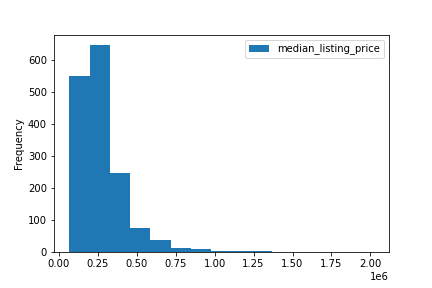
\includegraphics[width=.8\linewidth]{../data_and_processing/media/lst_prc_hist.png}
    \caption{Histogram for Median Listing Price \\ (Aggregate of 2016 and 2019)}
    \label{lst_prc_hist}
\end{figure*}

\begin{figure*}[h]
    \centering
    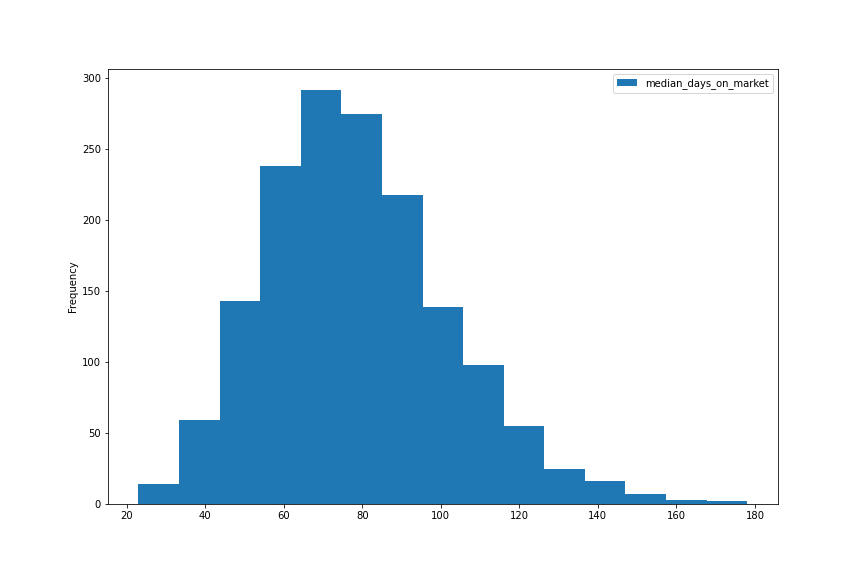
\includegraphics[width=.8\linewidth]{../data_and_processing/media/days_on_mkt_hist.png}
    \caption{Histogram for Median Days on Market \\ (Aggregate of 2016 and 2019)}
    \label{days_on_mkt_hist}
\end{figure*}

\begin{figure}[h]
    \centering
    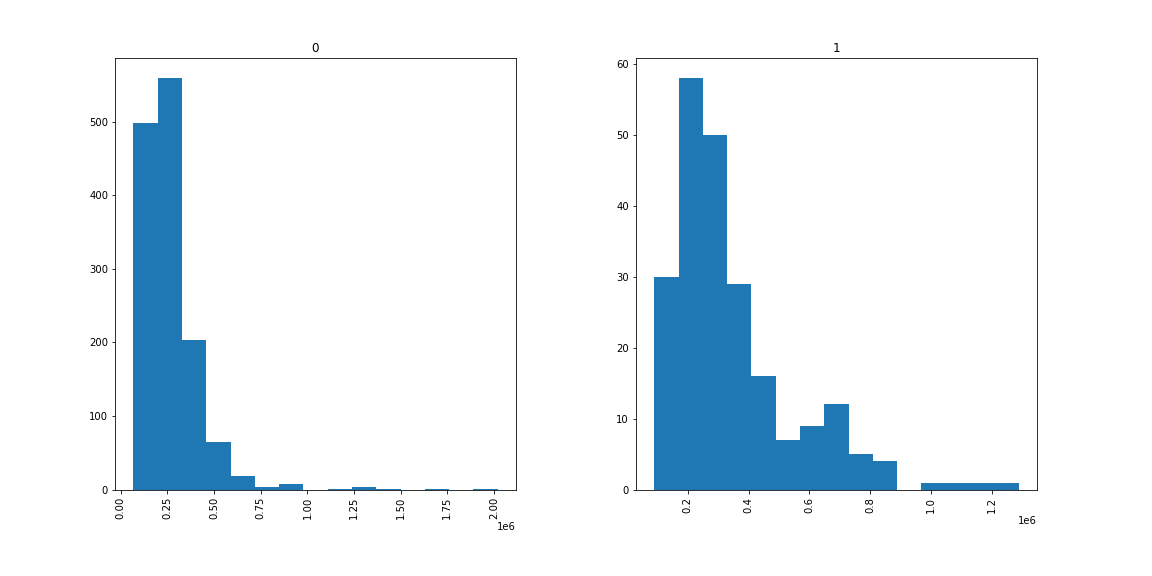
\includegraphics[width=.8\linewidth]{../data_and_processing/media/lst_prc_hist_comp.png}
    \caption{Control/Treatment Comparisson for Median Listing Price}
    \label{lst_prc_hist_comp}
\end{figure}

\begin{figure}[h]
    \centering
    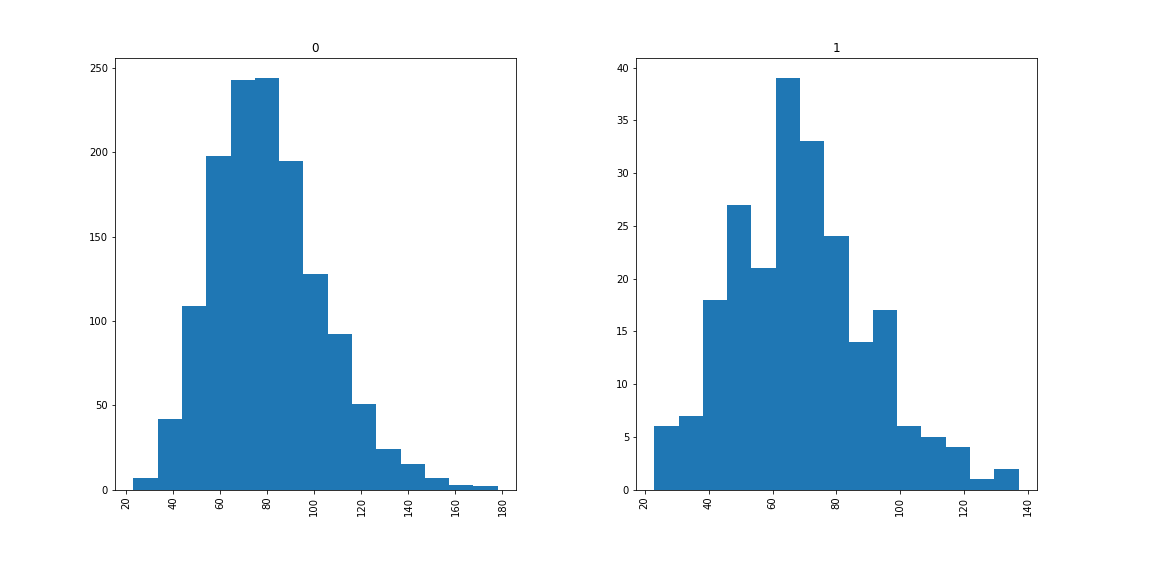
\includegraphics[width=.8\linewidth]{../data_and_processing/media/days_on_mkt_hist_comp.png}
    \caption{Control/Treatment Comparisson for Median Days on Market}
    \label{days_on_mkt_hist_comp}
\end{figure}
